%%%%% Elektrisches Feld %%%%%
%% #3 Kondensator %%


%Some sample text to be displayed above the first subsection

%\subsection{Prinzip}

%Ein Zyklotron besteht aus Zwei hohlen, halbzylindrischen und Duanden an denen eine Spannung mit unterschiedlichem Vorzeichen anliegt, und darüber bzw. darunter liegende Magneten, die ein homogenes Magnetfeld erzeugen. Zudem gibt es einen Einlass und einen Auslass für Teilchen.

%\begin{wrapfigure}{r}{0.4\textwidth} \label{Zyklo}
%
%	\vspace{-10pt}
%	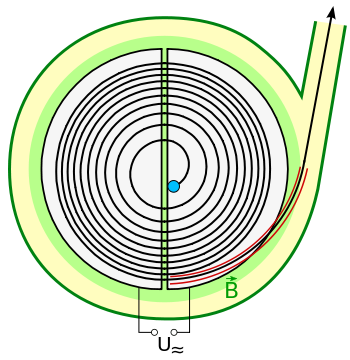
\includegraphics[width=0.35\textwidth]{Zyklotron_Prinzipskizze02.png}
%	\vspace{-13pt}
%	\caption{Prinzipskizze eines Zyklotrons}
%	\vspace{-5pt}	
%	
%\end{wrapfigure}

%\subsubsection{Anwendung}

% Some Formula:

%\begin{equation}
%	x= \frac{y \cdot 13 \pi z}
%			{\cos \alpha}
%\end{equation}

%%%%%%%%%%%%%%%%%%%%%%%
% Eigentlicher Beginn %
%%%%%%%%%%%%%%%%%%%%%%%

Der Plattenkondensator (im Folgenden nur noch Kondensator genannt) ist ein wichtiges Element der Elektrotechnik. Auch eignet er sich seht gut, um in der Schulphysik verschiedene Aspekte von elektrischen Feldern zu zeigen.


\subsection{Definition} \label{subsec:kon_def}

\begin{figure}[h!]
	\centering
	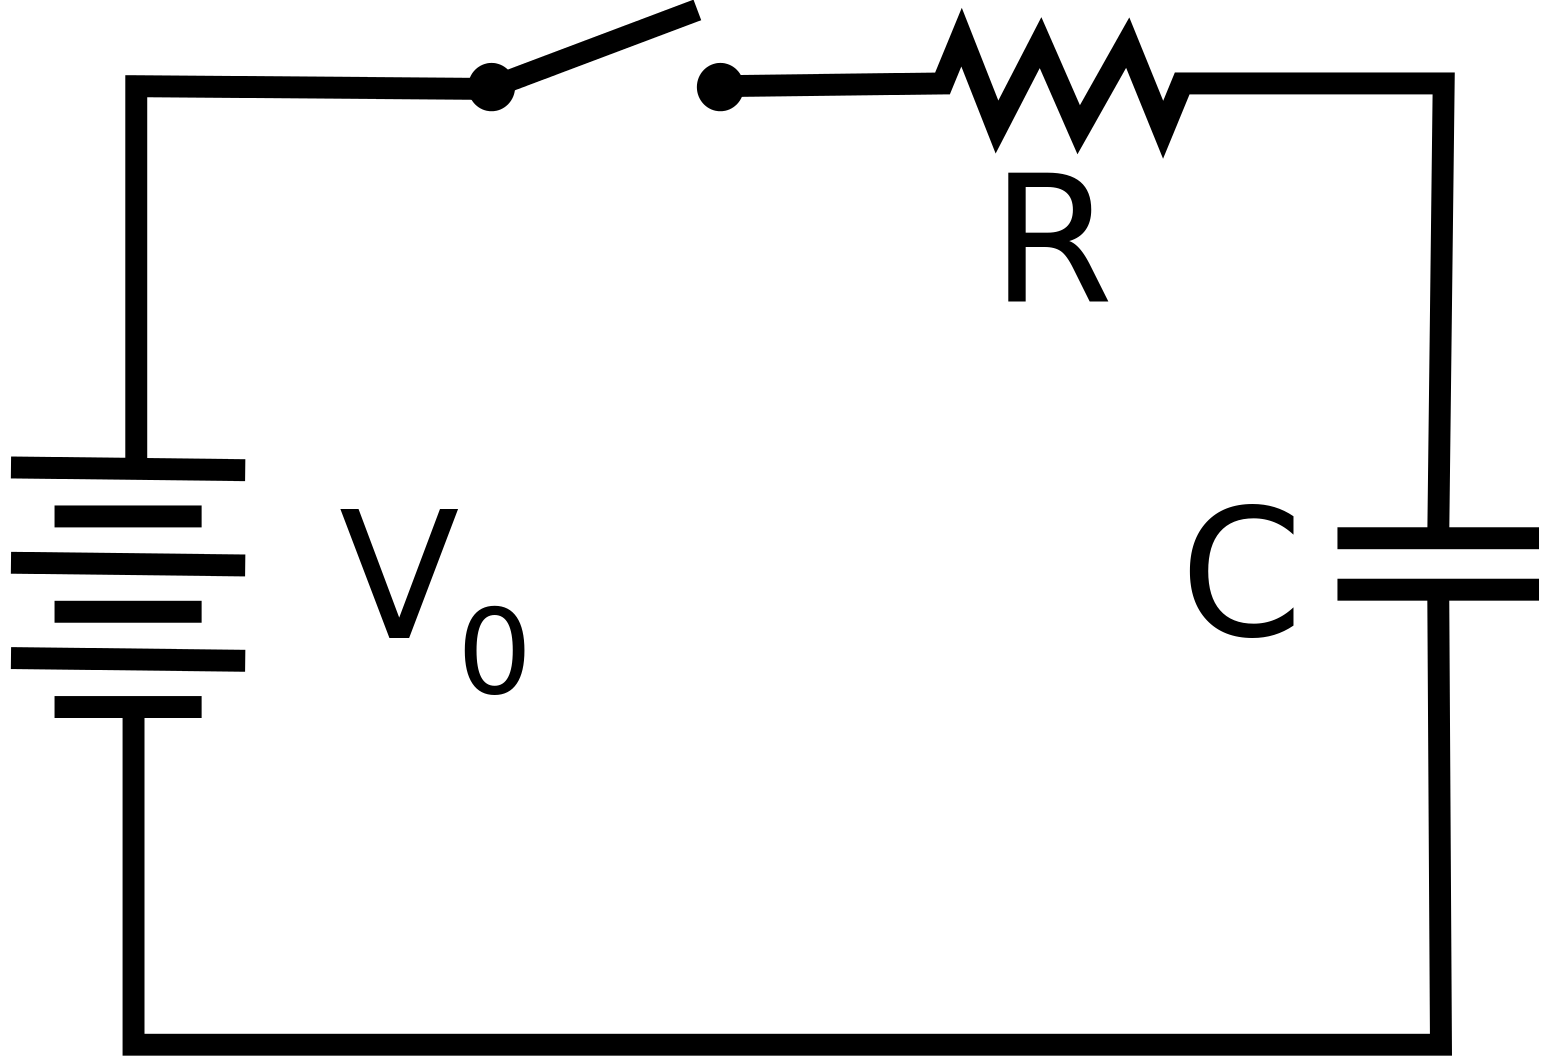
\includegraphics[width=0.6\textwidth]{RCWiring}
	\caption{Ein Schaltkreis mit Kondensator $C$ und Widerstand $R$}
	\label{fig:CapWiring}
\end{figure}

Ein Plattenkondensator besteht aus zwei ungleichnamig geladenen Platten, die sich parallel gegenüberstehen. Sie sind an ein Spannungsquelle angeschlossen. In einem Schaltplan wird er wie in Abbildung \ref{fig:CapWiring} \footnote{"RC switch" by PureCore - Own work. Licensed under CC BY-SA 3.0 via Commons - \url{https://commons.wikimedia.org/wiki/File:RC_switch.svg}} notiert.

\begin{Wichtig}
An sich fließt kein Strom durch den Kondensator! Die Platten sind elektrisch getrennt; das Dielektrikum, also das nicht-leitende Material zwischen den Platten (z.B. Luft), isoliert. 
\end{Wichtig}


\subsection{Elektrisches Feld im Inneren des Kondensators}

\begin{figure}[h!]
	\centering
	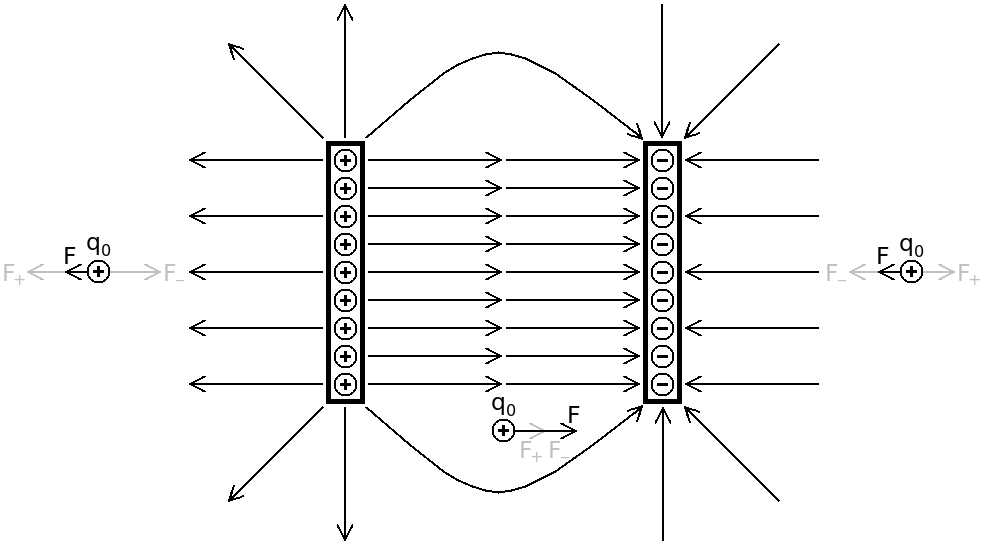
\includegraphics[width=\textwidth]{EFeldKondensator}
	\caption{Das elektrische Feld in und um einen Plattenkondensator}
\end{figure}

Durch den Überschuss positiver Ladungen auf der einen Seite und negativer Ladungen auf der Anderen, ergibt sich ein homogenes Magnetfeld zwischen den Platten.\footnote{„E Feld Kondensator“. Über Wikibooks - \url{https://de.wikibooks.org/wiki/Datei:E_Feld_Kondensator.png}}

\subsubsection{Feldstärke}

Die Stärke des Feldes im Inneren lässt sich auf recht einfach Art aus der anliegenden Spannung $U$ und dem Plattenabstand $d$ berechnen:

\begin{equation} \label{eq:feldstaerke_kondensator}
	E = \frac{U}{d}
\end{equation}

Die resultierende Einheit $\frac{V}{m}$ ist äquivalent zu $\frac{N}{C}$, der generellen Einheit für die Feldstärke (Siehe \referenz{subsec:Feldstaerke}).

\begin{Aufgabe}
Zeige, dass $\frac{V}{m}$ äquivalent zu $\frac{N}{C}$ ist, indem Du die Definitionen der Einheiten Volt $V=\frac{kg \cdot m^2}{A \cdot s^3}$, Newton und Coulomb einsetzt.

Einheitenrechnungen sind praktisch, um Ansätze für Herleitungen zu verifizieren. Am Ende muss auch immer die richtige Einheit für eine Größe aus den Größen in der Formel herauskommen.

Der Leser fühle sich hiermit eingeladen, eine Einheitenrechnung für jede hier aufgeführte Gleichung anzustellen. 
\end{Aufgabe}

\subsubsection{Kraft auf Körper}

In die allgemeine Gleichung für eine Kraft auf einen geladenen Körpern (Gleichung \ref{eq:feldstaerke_nach_F} auf Seite \pageref{eq:feldstaerke_nach_F}: $\vec{F} = q \cdot \vec{E}$) kann nun die obige Gleichung für $E$ im Kondensator eingesetzt werden (Gleichung \ref{eq:feldstaerke_kondensator}):

\begin{equation} \label{eq:kraft_kondensator}
	F = q \cdot \frac{U}{d}
\end{equation}

In diesem Fall kann sowieso auf eine Vektorrechnung verzichtet werden, da die Richtung der des elektrischen Felds klar und das Feld homogen ist.

\subsubsection{Energieumsatz bei einer Bewegung eines Körpers}

Wenn ein Körper in einem Kondensator bewegt wird, wird dabei Energie umgesetzt. Eine äquivalente Ausdrucksweise wäre, es wird \glqq Arbeit verrichtet\grqq . Das geschieht gemäß dieser Formel, bei der $s$ die Strecke ist, um die der Körper verschoben wird:

\begin{equation} \label{eq:arbeit}
	W = F \cdot s
\end{equation}

\noindent Die Kraft $F$ kann durch Umstellen mit $F = q \cdot E$ zu

\begin{equation} \label{eq:arbeit_kondensator}
	W = q \cdot E \cdot s
\end{equation}

\noindent ersetzt werden.

\begin{NiceToKnow}
$W = q \cdot E \cdot s$ ist analog zur Lagearbeit aus der Mechanik: $W_{pot} = m \cdot g \cdot h$
\end{NiceToKnow}


\subsection{Flächenladungsdichte}

Die elektrische Feldstärke im Inneren eines Kondensators lässt sich auch über die Flächenladungsdichte berechnen. Die Flächenladungsdichte $\sigma$ (Spricht: \glqq klein Sigma\grqq ) gibt an, wie \emph{dicht} Ladungen auf den Kondensatorplatten verteilt sind:

\begin{equation} \label{eq:flaechenladungsdichte}
	\sigma = \frac{Q}{A}
\end{equation}

\begin{NiceToKnow}
Man schreibt $q$ für eine spezifische, unveränderbare Ladung eines Probekörpers und $Q$ für z.B. die Ladung von Kondensatorplatten oder den Betrag eines Ladungsflusses durch einen Leiter.
\end{NiceToKnow}

Die Flächenladungsdichte ist im homogenen Feld proportional zur Feldstärke ($\sigma \sim E$). Die Proportionalitätskonstante hierbei ist $\frac{1}{\epsilon_0}$ (Siehe \referenz{subsec:CoulombGesetz}), sodass sich ergibt:

\begin{equation} \label{eq:feldstaerke_mit_sigma}
	E = \frac{\sigma}{\epsilon_0} = \frac{1}{\epsilon_0} \cdot \frac{Q}{A}
\end{equation}

\subsubsection{Exkurs: Flächenladungsdichte bei Kugeln}

Die Oberfläche von Kugeln ist als $A=4\pi \cdot r^2$ definiert. Daher ergibt sich ein Spezialfall für die Feldstärke:

\begin{equation} \label{eq:feldstaerke_kugel}
	E = \frac{1}{\epsilon_0} \cdot \frac{Q}{4\pi \cdot r^2} = \frac{1}{4\pi \cdot \epsilon_0} \cdot \frac{Q}{r^2}
\end{equation}

Es fällt eine Ähnlichkeit mit dem Coulomb-Gesetz (Gleichung \gleichungsreferenz{eq:coulomb_gesetz}) auf, welches die Kraft zwischen zwei geladenen, sphärischen Körpern angibt.


\subsection{Kapazität des Kondensators}

Die wichtigste elektrische Größe eines Kondensators ist die Kapazität $C$ mit Einheit \glqq Farad\grqq{}, Zeichen $F = \frac{A \cdot s}{V} = \frac{A^2 \cdot s^4}{kg \cdot m^2} = \frac{A^2 \cdot s^2}{N \cdot m}$:

\begin{equation} \label{eq:kapazitaet}
	C = \frac{Q}{U}
\end{equation}

Die Kapazität gibt also an, wie viel Ladung ein Kondensator bei einer definierten Spannung fasst, bzw. wie hoch die Spannung sein muss, damit die definierte Ladung $Q$ auf den Kondensator \glqq geht\grqq .

Für eine Bestimmungsgleichung, welche nur aus Kenngrößen besteht, muss $Q$ ersetzt werden. Mit den beiden Definitionen für die Feldstärke ($E = \frac{\sigma}{\epsilon_0}$ und $E=\frac{U}{d}$) ergibt sich für $Q$:

\begin{align}
\begin{split}
	E = \frac{\sigma}{\epsilon_0} \\
	E = \frac{Q}{A \cdot \epsilon_0} \\
	\frac{U}{d} = \frac{Q}{A \cdot \epsilon_0} \\
	Q = \epsilon_0 \cdot \frac{U \cdot A}{d}
\end{split}
\end{align}

\noindent Dieses $Q$ lässt sich in die Gleichung für $C$ einsetzen:

\begin{equation}
	C = \epsilon_0 \cdot \frac{U \cdot A}{d \cdot U} = \epsilon_0 \epsilon_r \cdot \frac{A}{d}
\end{equation}

Die Spannung $U$ kürzt sich und es wurde ein weitere Konstante $\epsilon_r$ eingeführt. Die \glqq relative Feldkonstante\grqq{} charakterisiert die verstärkenden oder schwächenden Eigenschaften des Dielektrikum (\referenz{subsec:kon_def}). Für Luft bzw. Vakuum ist sie $\approx 1$. Es gibt jedoch Materialien, die durch eine hohe relative Feldkonstante die Kapazität um Faktoren bis ca. $10^3$ erhöhen.

\begin{NiceToKnow}
$BaTiO_3$, Bariumthiooxid, hat eine $\epsilon_r$ von $10^2-10^3$\footnote{Aus: \url{http://www.techniklexikon.net/d/dielektrizitaetskonstante/dielektrizitaetskonstante.htm}}
\end{NiceToKnow}


\subsection{Verschaltung von Kondensatoren}

\subsubsection{Parallel}

\begin{figure}[h!]
	\centering
	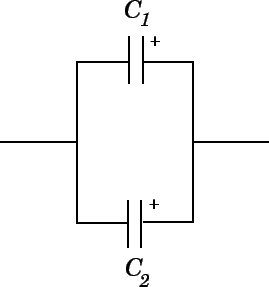
\includegraphics[width=0.5\textwidth]{CapsParallel}
	\caption{Parallelschaltung zweier Kapazitäten (= Kondensatoren) $C_1$ und $C_2$}
\end{figure}

Wenn Kondensatoren in einem Stromkreis parallel\footnote{Abbildung von: \url{http://farside.ph.utexas.edu/teaching/302l/lectures/node46.html}} geschaltet werden, addieren sich die Kapazitäten. Man kann sagen, dass die effektive Platte größer wird und daher mehr Ladung pro Spannung tragen kann (Siehe \gleichungsreferenz{eq:kapazitaet}):

\begin{equation}
	C_{ges} = \sum\limits_{i=1}^n C_i = C_1 + C_2 + \cdots + C_n
\end{equation}

\noindent Die Spannung bleibt dann aufgrund derselben Beziehung an jedem Element konstant:

\begin{equation}
	U_{ges} = U_1 = U_2 = \cdots = U_n
\end{equation}


\subsubsection{In Reihe}

\begin{figure}[h!]
	\centering
	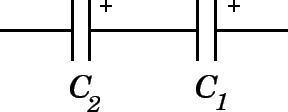
\includegraphics[width=0.5\textwidth]{CapsSeries}
	\caption{Reihenschaltung zweier Kapazitäten (= Kondensatoren) $C_1$ und $C_2$}
\end{figure}

Wenn Kondensatoren in einem Stromkreis in Reihe\footnote{Abbildung von: \url{http://farside.ph.utexas.edu/teaching/302l/lectures/node46.html}} geschaltet werden, ist die Summe der Kehrwerte der einzelnen Kapazitäten der Kehrwert der Gesamtkapazität. Das liegt daran, dass das \glqq Mittelstück\grqq , also die positive Plattes von $C_1$ und die negative Platte von $C_2$, ein definierte Ladung tragen, das heißt die positiven und negativen Ladungen können nur durch Influenz (Siehe \referenz{subsec:Influenz}) auftreten, da dieses Stück elektrisch vom Rest des Schaltkreises, also auch von einer mögliches Ladungsquelle getrennt ist.

Daher ist die Gesamtkapazität der Schaltung $0F$, wenn einer der beiden Kondensatoren die Kapazität $0F$ hat; $0,5F$, wenn beide Kondensatoren die Kapazität $1F$ haben; und die Gesamtkapazität kann nie größer sein als die niedrigste Einzelkapazität in der Kondensatorschaltung.

\begin{equation}
	\frac{1}{C_{ges}} = \sum\limits_{i=1}^n \frac{1}{C_i} = \frac{1}{C_1} + \frac{1}{C_2} + \cdots + \frac{1}{C_n}
\end{equation}

\noindent Wie auch bei der Reihenschaltung von Widerständen oder Spannungsquellen, addieren sich die Spannungen an den einzelnen Elementen zur Gesamtspannung:

\begin{equation}
	U_{ges} = \sum\limits_{i=1}^n U_i = U_1 + U_2 + \cdots + U_n
\end{equation}

